\chapter{Análisis de Requerimientos}
\label{ch:requerimientos}

\begin{chapterabstract}
Este capítulo traduce el problema precisado por el \textit{User Research} (Capítulo~\ref{ch:user_research}) en \textbf{12 Historias de Usuario}, con sus criterios de aceptación, \textbf{17 Requerimientos Funcionales} y \textbf{11 Requerimientos No Funcionales}, cada uno con su trazabilidad de origen. Se definen además los dos actores funcionales del proyecto (Estudiante y Docente/Evaluador) y las exclusiones que delimitan el alcance del MVP.
\end{chapterabstract}

El análisis de requerimientos de ImprontIA se estructura mediante Historias de Usuario, Requerimientos Funcionales y Requerimientos No Funcionales. Esta organización permite mantener trazabilidad entre las necesidades funcionales de los actores, las capacidades esperadas del sistema y las condiciones de calidad aplicables a la solución, sin anticipar decisiones tecnológicas o de arquitectura.

\section{Actores funcionales}
\label{sec:actores}

El sistema considera dos actores funcionales:

\begin{description}
    \item[Estudiante] actor que realiza la evaluación y recibe previamente la información sobre supervisión, reglas y recursos permitidos.
    \item[Docente/Evaluador] actor que revisa sesiones, evidencia contextualizada e indicadores, manteniendo el juicio académico humano.
\end{description}

\section{Exclusiones del alcance}

\begin{keyfinding}{Fuera del alcance del MVP}
\begin{itemize}
    \item ImprontIA no es un LMS ni un editor completo de evaluaciones.
    \item El mecanismo técnico para asociar o recibir el contexto de una evaluación que se administra en otra plataforma no forma parte del MVP.
    \item ImprontIA puede indicar que una situación requiere validación adicional, pero no ejecuta el mecanismo de validación.
    \item No se implementa enrolamiento biométrico individual (no se construye un perfil de referencia propio por estudiante): la estrategia de comparación adoptada para el MVP es una línea base poblacional, descripta en la Sección~\ref{sec:procesamiento_ia}.
    \item El sistema no captura contenido exacto del portapapeles, \textit{screenshots}, video de cámara ni audio de micrófono, y no registra los sitios externos visitados fuera de la aplicación de evaluación.
    \item No se implementa \textit{fingerprinting} complejo de navegador o dispositivo, ni se utiliza la dirección IP como señal de fraude.
    \item ImprontIA no intenta detectar de forma explícita el uso de ChatGPT u otro generador de texto, ni clasificar automáticamente interacción humana frente a un agente de IA: el sistema reporta atipicidad conductual relativa a la muestra, no atribución de autoría no humana (Sección~\ref{sec:procesamiento_ia}).
\end{itemize}
\end{keyfinding}

\section{Historias de Usuario}

\begin{description}[leftmargin=0cm, style=nextline]
\item[\textbf{HU01 --- Información previa sobre la supervisión}] Como estudiante, quiero conocer antes de iniciar la evaluación qué información será registrada y con qué finalidad, para comprender las condiciones bajo las cuales voy a rendir.
\item[\textbf{HU02 --- Reglas y condiciones de la evaluación}] Como estudiante, quiero conocer las reglas y los recursos permitidos para la evaluación, para saber qué se espera de mí durante su realización.
\item[\textbf{HU03 --- Captura proporcional de señales}] Como estudiante, quiero que durante la evaluación se registren únicamente las señales previamente informadas y necesarias, para rendir sin interferencias innecesarias y comprender el alcance de la supervisión.
\item[\textbf{HU04 --- Contexto de la evaluación}] Como docente, quiero que cada sesión conserve el contexto relevante de la evaluación, para interpretar correctamente las señales registradas.
\item[\textbf{HU05 --- Identificación de sesiones para revisión}] Como docente, quiero identificar qué sesiones presentan eventos o patrones que requieren mi atención, para concentrar la revisión en los casos más relevantes.
\item[\textbf{HU06 --- Revisión de evidencia contextualizada}] Como docente, quiero consultar las señales, métricas e indicadores asociados a una sesión junto con su contexto, para comprender por qué requiere atención antes de emitir una valoración académica.
\item[\textbf{HU07 --- Revisión humana}] Como docente, quiero revisar personalmente los indicadores de una sesión antes de que puedan asociarse con una decisión académica, para conservar el juicio académico humano y considerar posibles explicaciones alternativas.
\item[\textbf{HU08 --- Validación adicional}] Como docente, quiero poder indicar que una situación requiere una validación adicional cuando la evidencia disponible no sea suficiente, para profundizar el caso antes de adoptar una decisión académica.
\item[\textbf{HU09 --- Configuración de la evaluación}] Como docente, quiero definir para cada evaluación la información previa, las reglas, la consigna y las señales que se registrarán, para adecuar la supervisión al objetivo de esa evaluación.
\item[\textbf{HU10 --- Participación sin identificación directa}] Como estudiante, quiero rendir identificándome con un código de participante y sin crear una cuenta, para que mis registros de interacción no queden asociados directamente a mi identidad dentro de la plataforma.
\item[\textbf{HU11 --- Panorama de la evaluación}] Como docente, quiero consultar un panorama agregado del proceso de una evaluación completa, interpretado según las reglas que definí para ella, para comprender cómo se desarrolló la evaluación aunque ninguna sesión requiera revisión.
\item[\textbf{HU12 --- Eliminación de los datos}] Como estudiante, quiero poder solicitar la eliminación de los registros de mi sesión, y como docente, quiero poder eliminar mi cuenta junto con las evaluaciones que administro, para que la información conductual no se conserve más allá de su finalidad.
\end{description}

\section{Criterios de aceptación de las Historias de Usuario}
\label{sec:criterios_aceptacion}

Cada Historia de Usuario se acompaña de un criterio de aceptación en formato \textit{dado / cuando / entonces}, que expresa la condición observable con la que se considera satisfecha (Tabla~\ref{tab:criterios_aceptacion}).

{\small
\begin{longtable}{>{\raggedright\arraybackslash}p{1.1cm} >{\raggedright\arraybackslash}p{3.3cm} >{\raggedright\arraybackslash}p{3.3cm} >{\raggedright\arraybackslash}p{5.6cm}}
    \caption{Criterios de aceptación de las Historias de Usuario}\label{tab:criterios_aceptacion}\\
    \toprule
    \tblhead \textbf{HU} & \textbf{Dado} & \textbf{Cuando} & \textbf{Entonces} \\
    \midrule
    \endfirsthead
    \toprule
    \tblhead \textbf{HU} & \textbf{Dado} & \textbf{Cuando} & \textbf{Entonces} \\
    \midrule
    \endhead
    HU01 & una evaluación con señales habilitadas & el estudiante ingresa con el código de acceso & ve qué señales se registran y para qué antes de poder iniciar, y la sesión registra su consentimiento. \\
    HU02 & una evaluación con reglas y recursos definidos & el estudiante ingresa a la evaluación & ve las reglas y los recursos permitidos antes de iniciar. \\
    HU03 & una evaluación con solo algunas señales habilitadas & el estudiante resuelve la evaluación & solo se almacenan eventos de las señales habilitadas. \\
    HU04 & una sesión finalizada & el docente abre su detalle & ve la versión de la política, las reglas y la consigna vigentes al iniciar la sesión. \\
    HU05 & un conjunto de sesiones procesadas & el docente abre el listado & distingue las sesiones que requieren revisión de las que no. \\
    HU06 & una sesión con indicadores & el docente abre su detalle & ve cada indicador con la métrica, el valor y el umbral o las métricas que lo originan. \\
    HU07 & una sesión con indicadores de nivel alto & finaliza el procesamiento & la sesión queda pendiente de revisión y ninguna decisión académica se registra sin una acción del docente. \\
    HU08 & una sesión en revisión & el docente marca que requiere validación adicional & la sesión figura en la vista de validaciones pendientes. \\
    HU09 & un docente autenticado & crea o modifica una evaluación & la configuración queda guardada como una versión nueva y las sesiones ya iniciadas conservan la anterior. \\
    HU10 & un estudiante con el código de acceso & inicia la evaluación & lo hace con un código de participante, sin crear una cuenta. \\
    HU11 & una evaluación con sesiones finalizadas & el docente abre el panorama & ve los valores típicos de las métricas y la cantidad de sesiones por tipo de indicador, interpretados según las reglas de la evaluación. \\
    HU12 & una solicitud de eliminación o un plazo de conservación vencido & el docente confirma la eliminación o se cumple el plazo & la información de la sesión, o de la cuenta y sus evaluaciones, deja de estar almacenada. \\
    \bottomrule
\end{longtable}
}

\section{Requerimientos Funcionales}

\begin{description}[leftmargin=0cm, style=nextline]
\item[\textbf{RF01 --- Información previa sobre el registro}] El sistema debe presentar al estudiante, antes de iniciar la evaluación, qué información y qué categorías de señales se registran y con qué finalidad se utilizan. \textit{HU de origen: HU01. Prioridad: Alta.}
\item[\textbf{RF02 --- Información sobre reglas y recursos permitidos}] El sistema debe presentar al estudiante, antes de iniciar la evaluación, las reglas aplicables y los recursos permitidos definidos para dicha instancia. \textit{HU de origen: HU02. Prioridad: Alta.}
\item[\textbf{RF03 --- Registro de señales durante la sesión}] El sistema debe registrar durante la sesión de evaluación las señales de interacción definidas para dicha instancia, asociándolas a la sesión correspondiente. \textit{HU de origen: HU03. Prioridad: Alta.}
\item[\textbf{RF04 --- Limitación de las señales registradas}] El sistema debe limitar el registro de la sesión a las señales previamente informadas al estudiante y definidas como necesarias para la evaluación. \textit{HU de origen: HU03. Prioridad: Alta.}
\item[\textbf{RF05 --- Conservación del contexto de la evaluación}] El sistema debe asociar y conservar para cada sesión el contexto relevante de la evaluación necesario para interpretar posteriormente las señales registradas. \textit{HU de origen: HU04. Prioridad: Alta.}
\item[\textbf{RF06 --- Identificación de sesiones que requieren revisión}] El sistema debe identificar las sesiones que presenten eventos, patrones o indicadores definidos como relevantes para su posterior revisión por parte del docente. \textit{HU de origen: HU05. Prioridad: Alta.}
\item[\textbf{RF07 --- Presentación de sesiones para revisión}] El sistema debe presentar al docente las sesiones disponibles, permitiendo distinguir aquellas que contienen eventos, patrones o indicadores que requieren su atención para revisión. \textit{HU de origen: HU05. Prioridad: Alta.}
\item[\textbf{RF08 --- Consulta de evidencia contextualizada}] El sistema debe permitir al docente consultar, para una sesión seleccionada, las señales, métricas e indicadores generados junto con el contexto relevante de la evaluación. \textit{HU de origen: HU06. Prioridad: Alta.}
\item[\textbf{RF09 --- Trazabilidad del origen de los indicadores}] El sistema debe permitir al docente relacionar cada indicador presentado con los eventos, señales o métricas que lo sustentan. \textit{HU de origen: HU06. Prioridad: Alta.}
\item[\textbf{RF10 --- Separación entre indicador y decisión académica}] El sistema debe someter a revisión humana toda interpretación de señales, métricas o indicadores, y debe exigir que cualquier valoración o decisión académica asociada a una sesión sea registrada explícitamente por un docente, de modo que las decisiones académicas resulten siempre de una acción humana. \textit{HU de origen: HU07. Prioridad: Alta.}
\item[\textbf{RF11 --- Indicación de validación adicional}] El sistema debe permitir al docente indicar que una situación requiere una validación adicional cuando considere que la evidencia disponible no resulta suficiente para adoptar una decisión académica. \textit{HU de origen: HU08. Prioridad: Media.}
\item[\textbf{RF12 --- Configuración de la evaluación y de la política de captura}] El sistema debe permitir al docente crear una evaluación y definir su información previa, sus reglas, su consigna y las categorías de señales habilitadas; cada modificación de esa configuración debe conservarse como una versión nueva, sin alterar las sesiones ya iniciadas. \textit{HU de origen: HU09. Prioridad: Alta.}
\item[\textbf{RF13 --- Participación seudónima del estudiante}] El sistema debe permitir que el estudiante acceda a una evaluación mediante un código de acceso e inicie su sesión con un código de participante seudónimo, sin requerir una cuenta en la plataforma. \textit{HU de origen: HU10. Prioridad: Alta.}
\item[\textbf{RF14 --- Acceso autenticado del docente}] El sistema debe exigir que el docente se autentique para consultar sesiones, evidencia e indicadores, y debe limitar ese acceso a las evaluaciones que el propio docente administra. \textit{HU de origen: HU05, HU06. Prioridad: Alta.}
\item[\textbf{RF15 --- Panorama agregado de la evaluación}] El sistema debe presentar al docente, para cada evaluación que administra, un resumen agregado de las sesiones finalizadas: cantidad de sesiones y de sesiones que requieren revisión, valores típicos y dispersión de las métricas principales, sesiones por tipo de indicador y proporción de sesiones marcadas por el modelo poblacional, calculado a partir de las métricas e indicadores ya registrados. \textit{HU de origen: HU11. Prioridad: Media.}
\item[\textbf{RF16 --- Relevancia de los eventos según las reglas de la evaluación}] El sistema debe permitir al docente declarar, al configurar la evaluación, qué conductas están permitidas por sus reglas, y debe conservar el registro de los eventos correspondientes sin presentarlos como motivo de revisión cuando la regla los permita. \textit{HU de origen: HU09, HU05. Prioridad: Media.}
\item[\textbf{RF17 --- Eliminación de cuenta y de datos asociados}] El sistema debe permitir al docente eliminar su cuenta y, con ella, las evaluaciones que administra y todas sus sesiones, eventos, métricas, indicadores y revisiones; debe permitir además eliminar los registros de una sesión identificada por su código de participante cuando el estudiante lo solicite, y debe eliminar automáticamente la información de las sesiones al vencer el plazo de conservación de la política de captura (RNF10). \textit{HU de origen: HU12. Prioridad: Alta.}
\end{description}

\section{Requerimientos No Funcionales}

\begin{description}[leftmargin=0cm, style=nextline]
\item[\textbf{RNF01 --- Minimización y proporcionalidad de datos}] El sistema debe limitar la recolección y el tratamiento de datos a las señales necesarias para las finalidades previamente definidas para la evaluación, evitando la captura de información ajena a dicho propósito. \textit{Justificación: el marco teórico establece privacidad desde el diseño, minimización de la captura y limitación al entorno de evaluación; el User Research refuerza que la privacidad no depende únicamente de evitar cámara o micrófono, sino también de qué se captura, cuánto se captura y para qué se utiliza. Prioridad: Alta.}
\item[\textbf{RNF02 --- Transparencia del tratamiento de información}] El sistema debe presentar al estudiante información clara y comprensible sobre las categorías de datos registradas y su finalidad, generada a partir de la misma configuración que determina la captura efectivamente realizada durante la evaluación. \textit{Justificación: la transparencia previa constituye una de las condiciones con mayor respaldo del User Research (COM01: 93{,}0\,\% en niveles 4--5). Prioridad: Alta.}
\item[\textbf{RNF03 --- Protección y confidencialidad de la información}] El sistema debe proteger las señales, métricas, indicadores y demás información asociada a las sesiones frente a accesos, divulgaciones o modificaciones no autorizadas durante su tratamiento y conservación, mediante cifrado en tránsito (HTTPS con TLS), cifrado en reposo del almacenamiento de la base de datos, almacenamiento de las contraseñas docentes únicamente como \textit{hash} con una función adaptativa (\textit{bcrypt}), control de acceso por rol y por propietario de la evaluación, y seudonimización de los participantes. \textit{Justificación: ImprontIA procesa información conductual que puede vincularse con datos personales y, según su tratamiento, con características biométricas. Prioridad: Alta.}
\item[\textbf{RNF04 --- Integridad de los registros de sesión}] El sistema debe preservar la integridad y consistencia de los eventos y señales registrados durante una sesión, evitando que su contenido, asociación o secuencia puedan alterarse de manera no controlada. \textit{Justificación: la utilidad de ImprontIA depende de aportar trazabilidad sobre el proceso de producción de la respuesta. Prioridad: Alta.}
\item[\textbf{RNF05 --- Trazabilidad de la información procesada}] El sistema debe conservar trazabilidad suficiente entre la sesión, las señales registradas, las métricas obtenidas y los indicadores presentados, de forma que pueda reconstruirse el origen de la información utilizada durante una revisión. \textit{Justificación: la trazabilidad de autoría constituye el concepto central de ImprontIA y el RF09 exige relacionar los indicadores con las evidencias que los sustentan. Prioridad: Alta.}
\item[\textbf{RNF06 --- Explicabilidad de indicadores}] El sistema debe presentar los indicadores de manera interpretable, permitiendo comprender qué señales, eventos o métricas contribuyeron a su generación sin presentarlos como conclusiones automáticas sobre la conducta del estudiante. \textit{Justificación: el proyecto se define alrededor de información procesual, explicable y revisable; tanto el marco teórico como el User Research advierten que una señal puede ser ambigua. Prioridad: Alta.}
\item[\textbf{RNF07 --- Baja interferencia de la captura}] El sistema debe ejecutar la captura de señales de interacción de forma asíncrona y en segundo plano, de modo que el procesamiento de cada evento en el navegador se mantenga por debajo de 50\,ms y la escritura y la navegación de la evaluación conserven su fluidez normal, aun ante fallas transitorias de red. \textit{Justificación: la persona Santiago prioriza poder concentrarse en la evaluación sin fricción innecesaria, y las entrevistas describen cómo determinados mecanismos de supervisión pueden agregar presión al proceso. Prioridad: Alta.}
\item[\textbf{RNF08 --- Usabilidad para la revisión docente}] El sistema debe organizar y presentar la información de revisión de forma que el docente pueda localizar las sesiones relevantes, comprender su contexto e interpretar la evidencia asociada sin requerir un análisis innecesariamente complejo de los registros individuales. \textit{Justificación: la persona Laura necesita identificar situaciones relevantes, interpretar señales y utilizar su tiempo de revisión eficientemente. Prioridad: Alta.}
\item[\textbf{RNF09 --- Escalabilidad}] El sistema debe mantener su capacidad de registrar, procesar y presentar información ante incrementos en el volumen de sesiones y eventos, manteniendo los tiempos de respuesta del RNF11 para evaluaciones de hasta 500 sesiones y 200 sesiones simultáneas en curso. \textit{Justificación: la carga docente y la escalabilidad surgieron como consideración cualitativa exploratoria del User Research; la evidencia no permite aún establecer umbrales concretos, pero sí indica que generar más información no resulta útil si no puede gestionarse; las cotas se fijan como objetivo de diseño para una evaluación de cursada masiva. Prioridad: Media.}
\item[\textbf{RNF10 --- Conservación limitada de datos}] El sistema debe conservar las señales y demás información derivada de las sesiones únicamente durante el plazo de conservación definido en la política de captura de cada evaluación, que la institución fija según sus finalidades académicas y de revisión y que no puede superar los doce meses desde el cierre de la evaluación; vencido ese plazo, el sistema debe eliminar esa información (RF17). \textit{Justificación: el marco conceptual de privacidad utilizado por ImprontIA contempla finalidad específica, proporcionalidad y conservación limitada. Prioridad: Alta.}
\item[\textbf{RNF11 --- Tiempo de respuesta del procesamiento y de la revisión}] El sistema debe generar las métricas y los indicadores por reglas de una sesión en menos de 5\,s desde su finalización, y debe presentar al docente el listado de sesiones, el detalle de una sesión y el panorama de la evaluación en menos de 2\,s, para evaluaciones de hasta 500 sesiones. La inferencia del modelo de detección de anomalías se ejecuta una sola vez por evaluación, al cerrarla, sobre la cohorte completa; su tiempo se mide e informa por separado. \textit{Justificación: el indicador solo es útil si está disponible cuando el docente revisa; la latencia relevante es la del cálculo de métricas e indicadores, la del cierre de la evaluación y la de la consulta. Prioridad: Media.}
\end{description}

\section{Matriz de trazabilidad Historia de Usuario \texorpdfstring{$\rightarrow$}{->} Requerimiento Funcional}

\begin{table}[h!]
    \caption{Matriz de trazabilidad HU \texorpdfstring{$\rightarrow$}{->} RF}
    \label{tab:matriz_hu_rf}
    \centering
    \small
    \begin{tabularx}{\textwidth}{p{6.5cm} X}
        \toprule
        \tblhead \textbf{Historia de Usuario} & \textbf{Requerimientos Funcionales derivados} \\
        \midrule
        HU01 --- Información previa sobre la supervisión & RF01 \\
        HU02 --- Reglas y condiciones de la evaluación & RF02 \\
        HU03 --- Captura proporcional de señales & RF03, RF04 \\
        HU04 --- Contexto de la evaluación & RF05 \\
        HU05 --- Identificación de sesiones para revisión & RF06, RF07 \\
        HU06 --- Revisión de evidencia contextualizada & RF08, RF09 \\
        HU07 --- Revisión humana & RF10 \\
        HU08 --- Validación adicional & RF11 \\
        HU09 --- Configuración de la evaluación & RF12 \\
        HU10 --- Participación sin identificación directa & RF13 \\
        HU05, HU06 (acceso a la revisión) & RF14 \\
        HU11 --- Panorama de la evaluación & RF15 \\
        HU09, HU05 (relevancia según las reglas) & RF16 \\
        HU12 --- Eliminación de los datos & RF17 \\
        \bottomrule
    \end{tabularx}
\end{table}

La HU11 y los RF15 y RF16 extienden la propuesta de valor a la inteligencia sobre el proceso de evaluación (Sección~\ref{sec:impl_panorama}). La HU12 y el RF17, sobre la eliminación de cuentas y datos, dan soporte en la plataforma a los derechos del titular analizados en el Capítulo~\ref{ch:viabilidad} (Sección~\ref{sec:impl_retencion}).

\section{Aspectos a medir o verificar}

Los requerimientos no funcionales se traducen en los aspectos de medición o verificación de la Tabla~\ref{tab:rnf_medicion}; donde el requerimiento fija una cota cuantitativa (RNF07, RNF09, RNF10 y RNF11), esa cota es el criterio de aceptación. Los resultados obtenidos con el MVP se informan en los Capítulos~\ref{ch:implementacion} y~\ref{ch:evaluacion}; los aspectos que requieren participantes o un entorno de producción corresponden al piloto y a las etapas posteriores (Sección~\ref{sec:eval_piloto_futuro}).

\begin{table}[h!]
    \caption{Aspectos a medir o verificar por RNF}
    \label{tab:rnf_medicion}
    \centering
    \small
    \begin{tabularx}{\textwidth}{p{1.6cm} X}
        \toprule
        \tblhead \textbf{RNF} & \textbf{Aspecto a medir o verificar} \\
        \midrule
        \textbf{RNF01} & Correspondencia entre señales habilitadas, finalidad definida y datos efectivamente recolectados. \\
        \textbf{RNF02} & Comprensibilidad y correspondencia entre la información comunicada y la captura real. \\
        \textbf{RNF03} & Controles de acceso por rol y propietario, contraseñas almacenadas solo como \textit{hash} \textit{bcrypt}, HTTPS en el despliegue, cifrado en reposo del almacenamiento y pruebas de seguridad. \\
        \textbf{RNF04} & Consistencia de los registros, asociación correcta con la sesión y preservación de la secuencia de eventos. \\
        \textbf{RNF05} & Capacidad de reconstruir el origen de un indicador a partir de la sesión, las señales y las métricas asociadas. \\
        \textbf{RNF06} & Capacidad de un docente de interpretar el origen de un indicador a partir de la información presentada. \\
        \textbf{RNF07} & Tiempo de procesamiento de cada evento en el navegador (cota: 50\,ms) y continuidad de la escritura ante fallas de red. \\
        \textbf{RNF08} & Tiempo, esfuerzo y comprensión requeridos por el docente para localizar e interpretar sesiones relevantes. \\
        \textbf{RNF09} & Cumplimiento de las cotas del RNF11 en pruebas de carga con 500 sesiones por evaluación y 200 sesiones simultáneas. \\
        \textbf{RNF10} & Eliminación efectiva de la información de las sesiones al vencer el plazo de la política de captura (máximo: doce meses desde el cierre). \\
        \textbf{RNF11} & Tiempo entre la finalización de una sesión y la disponibilidad de sus indicadores por reglas (cota: 5\,s), tiempo del cierre de la evaluación con la inferencia del modelo sobre la cohorte (sin cota; se informa) y tiempo de respuesta de las consultas del docente (cota: 2\,s). \\
        \bottomrule
    \end{tabularx}
\end{table}

\section{Prototipo de interfaz (\textit{mockups})}
\label{sec:mockups}

A modo de cierre de este capítulo, se presentan capturas del prototipo de interfaz de ImprontIA, diseñado en Figma y organizado en dos flujos según los actores funcionales definidos en la Sección~\ref{sec:actores}: \textbf{Docente/Evaluador} (resumen de la evaluación, detalle de sesión y evidencia de producción) y \textbf{Estudiante} (transparencia previa al examen y pantalla de resolución). Estas pantallas materializan directamente los requerimientos funcionales listados más arriba: el resumen, el detalle de sesión y la evidencia de producción del docente corresponden a RF06--RF09, y la transparencia previa del estudiante corresponde a RF01--RF02.

\subsection{Flujo Docente}

\begin{figure}[h!]
    \centering
    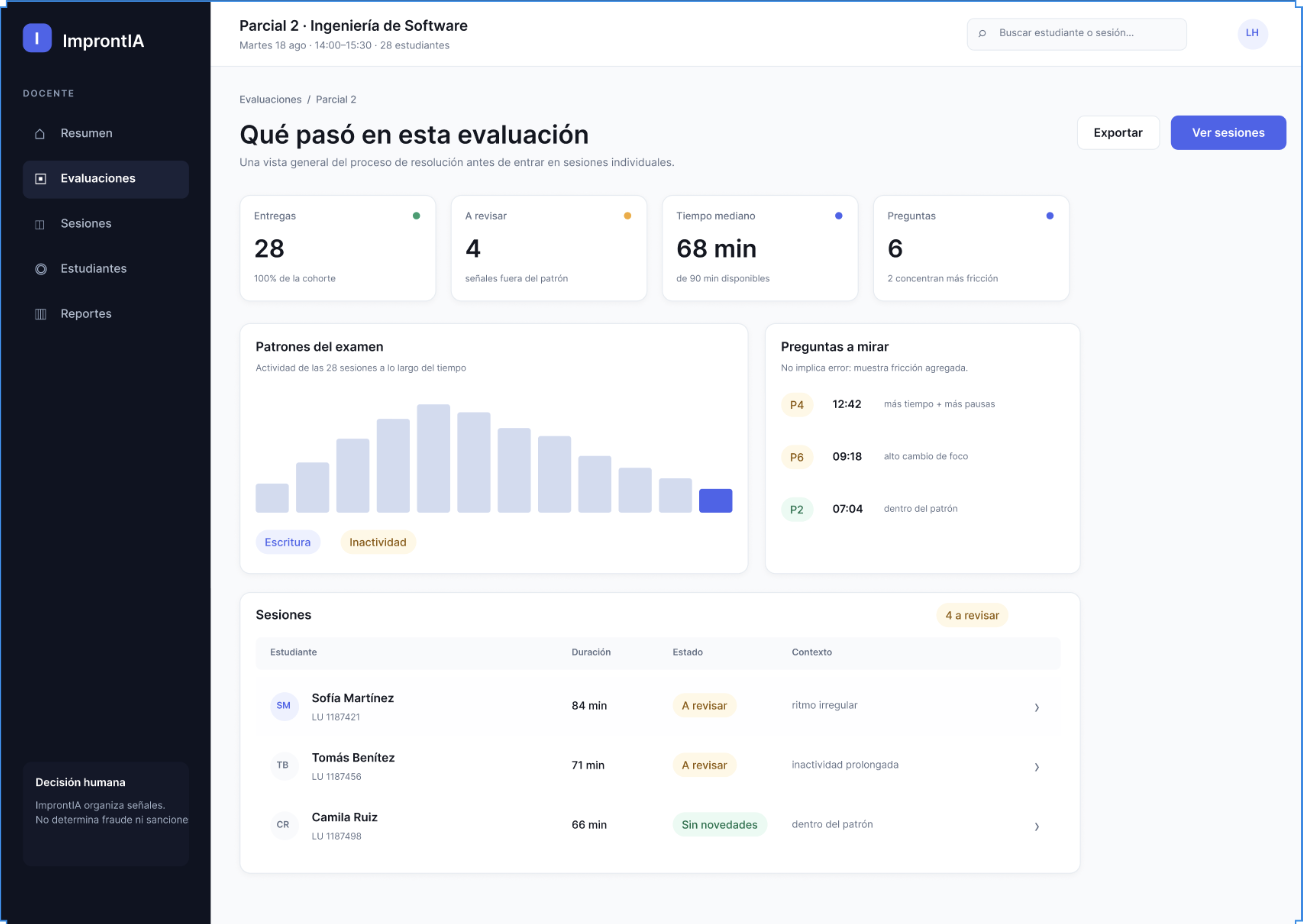
\includegraphics[width=0.85\textwidth]{./figures/mockup_docente_overview.png}
    \caption[Docente: resumen de la evaluación]{Docente. Resumen de la evaluación: entregas, sesiones a revisar y preguntas con mayor fricción agregada. Fuente: elaboración propia (prototipo diseñado en Figma).}
\end{figure}

\begin{figure}[h!]
    \centering
    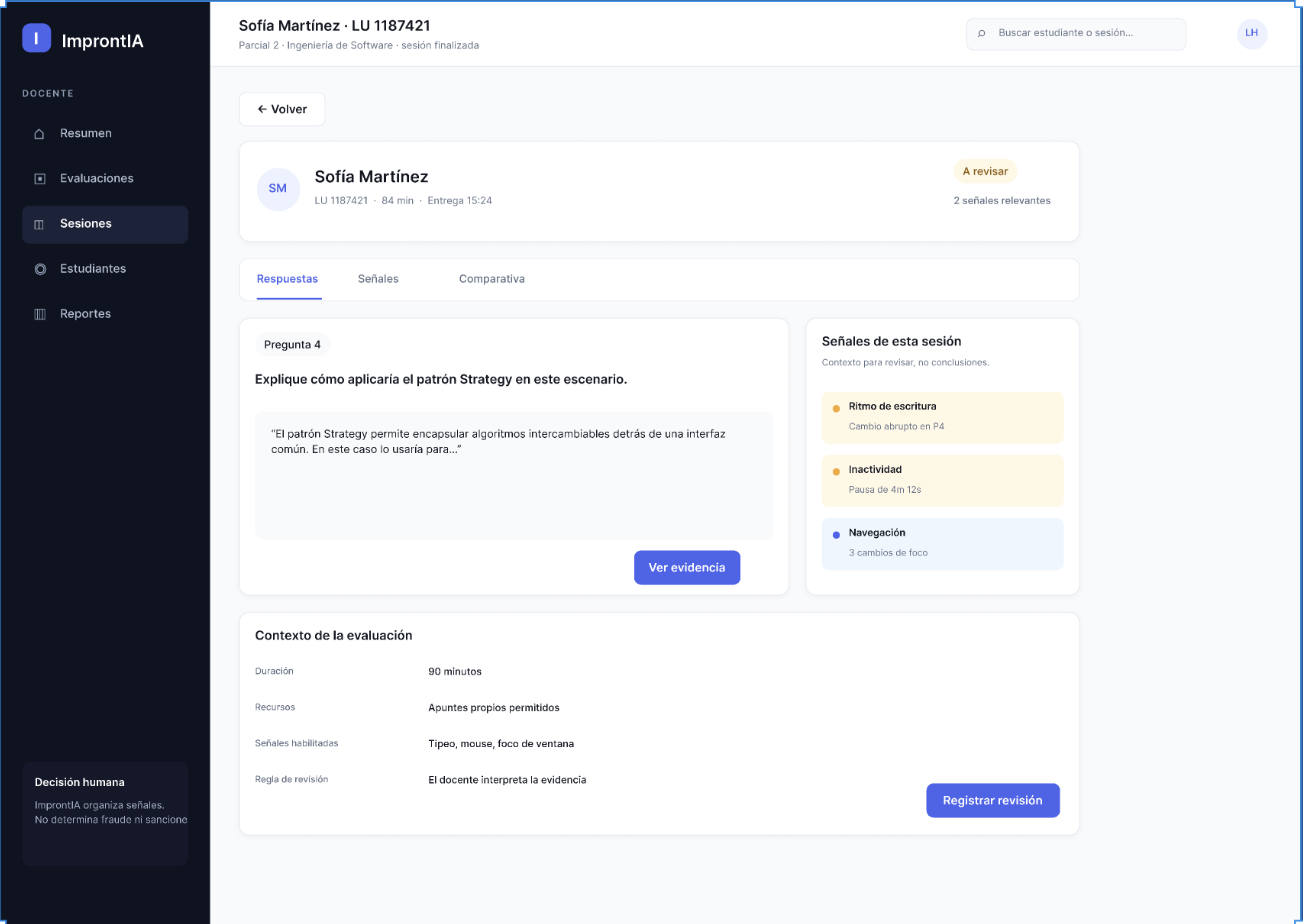
\includegraphics[width=0.85\textwidth]{./figures/mockup_docente_sesion.png}
    \caption[Docente: detalle de sesión de un estudiante, con señales registradas y contexto de la evaluación]{Docente. Detalle de sesión de un estudiante, con señales registradas y contexto de la evaluación. Fuente: elaboración propia (prototipo diseñado en Figma).}
\end{figure}

\clearpage
\begin{figure}[h!]
    \centering
    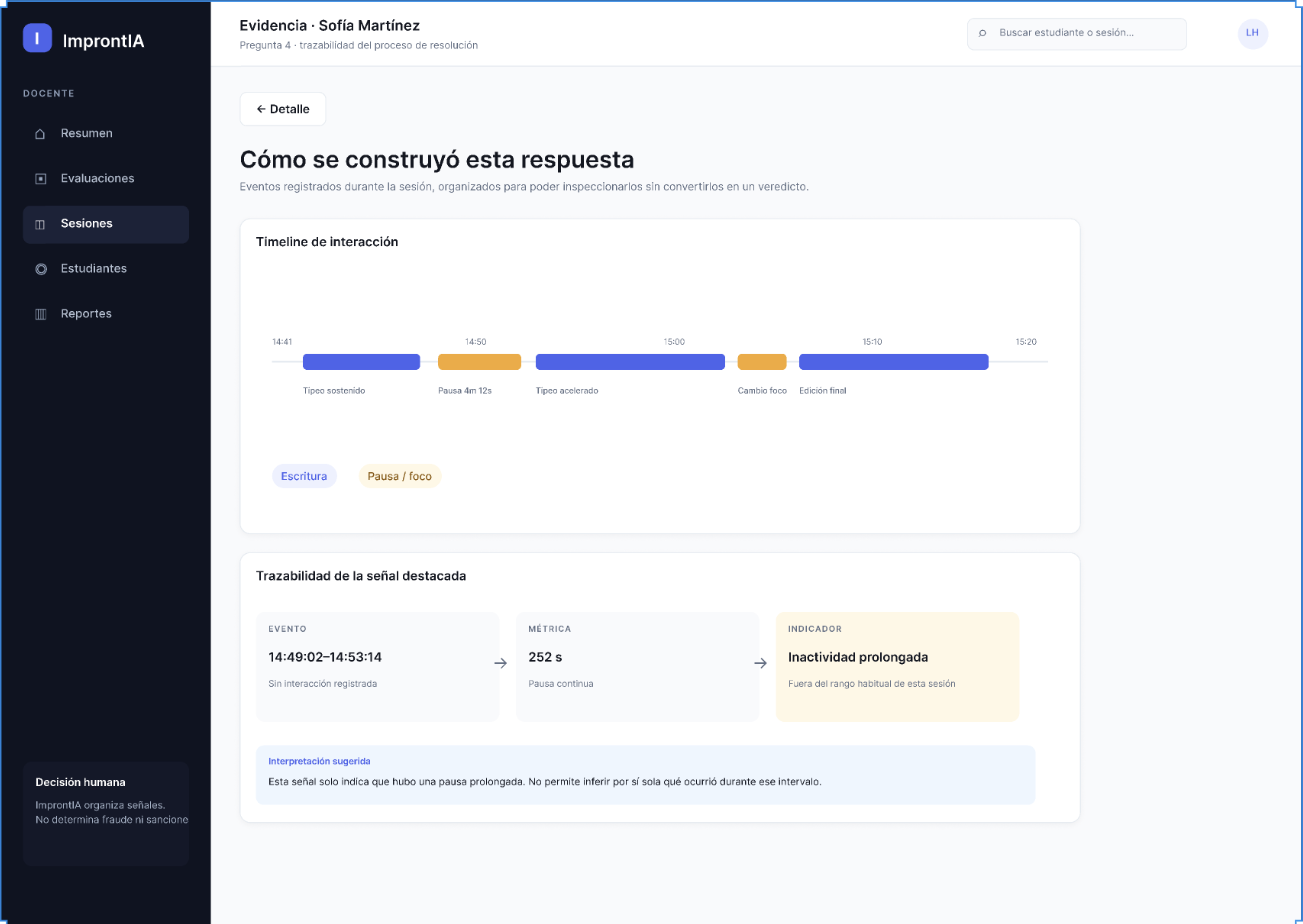
\includegraphics[width=0.85\textwidth]{./figures/mockup_docente_evidencia.png}
    \caption[Docente: evidencia de producción]{Docente. Evidencia de producción: \textit{timeline} de interacción y trazabilidad evento~$\rightarrow$~métrica~$\rightarrow$~indicador de una señal destacada. Fuente: elaboración propia (prototipo diseñado en Figma).}
\end{figure}

\clearpage
\subsection{Flujo Estudiante}

\begin{figure}[h!]
    \centering
    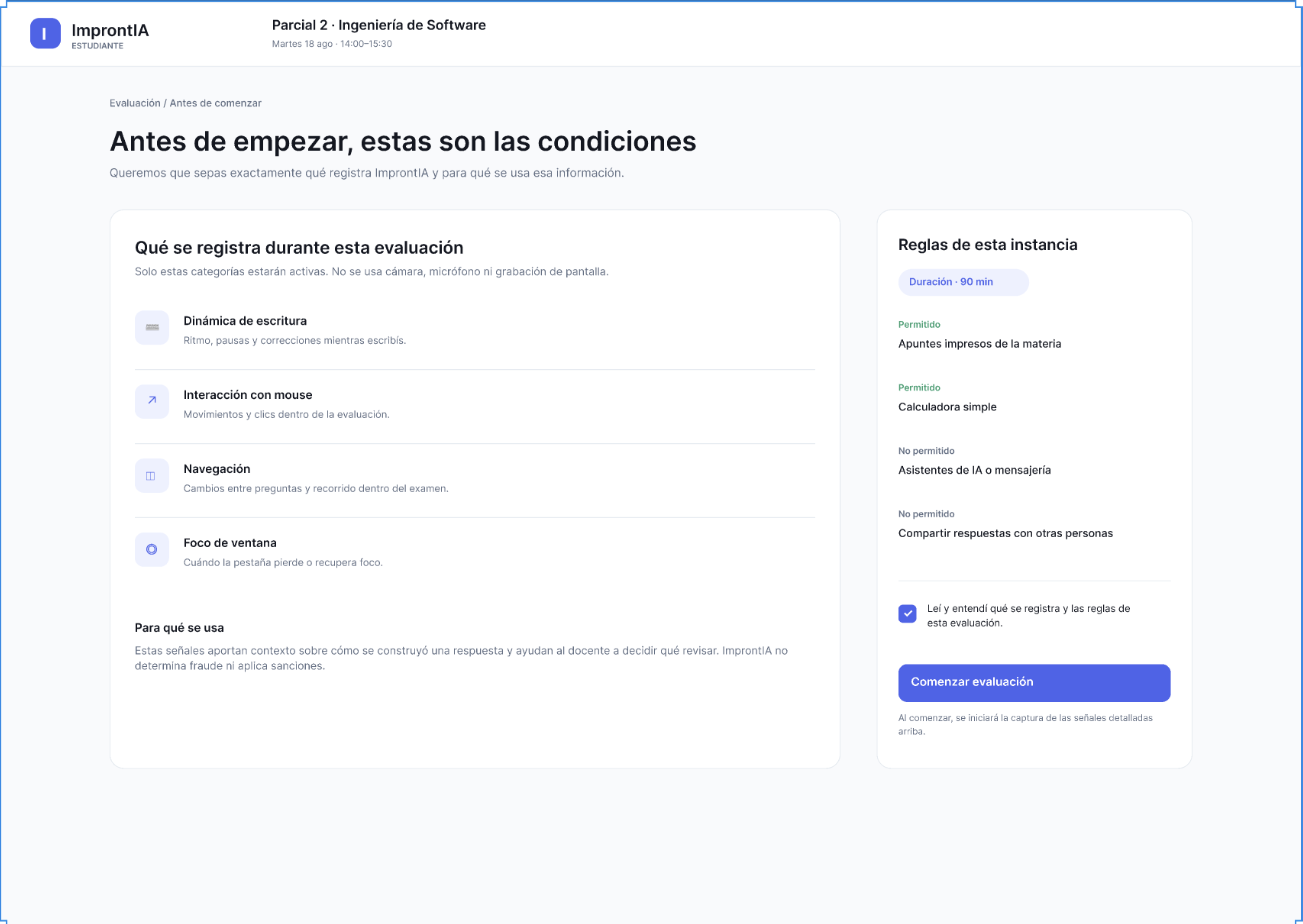
\includegraphics[width=0.85\textwidth]{./figures/mockup_estudiante_reglas.png}
    \caption[Estudiante: transparencia previa al examen]{Estudiante. Transparencia previa al examen: qué señales se registran, para qué se usan y reglas de la instancia. Fuente: elaboración propia (prototipo diseñado en Figma).}
\end{figure}

\clearpage
\begin{figure}[h!]
    \centering
    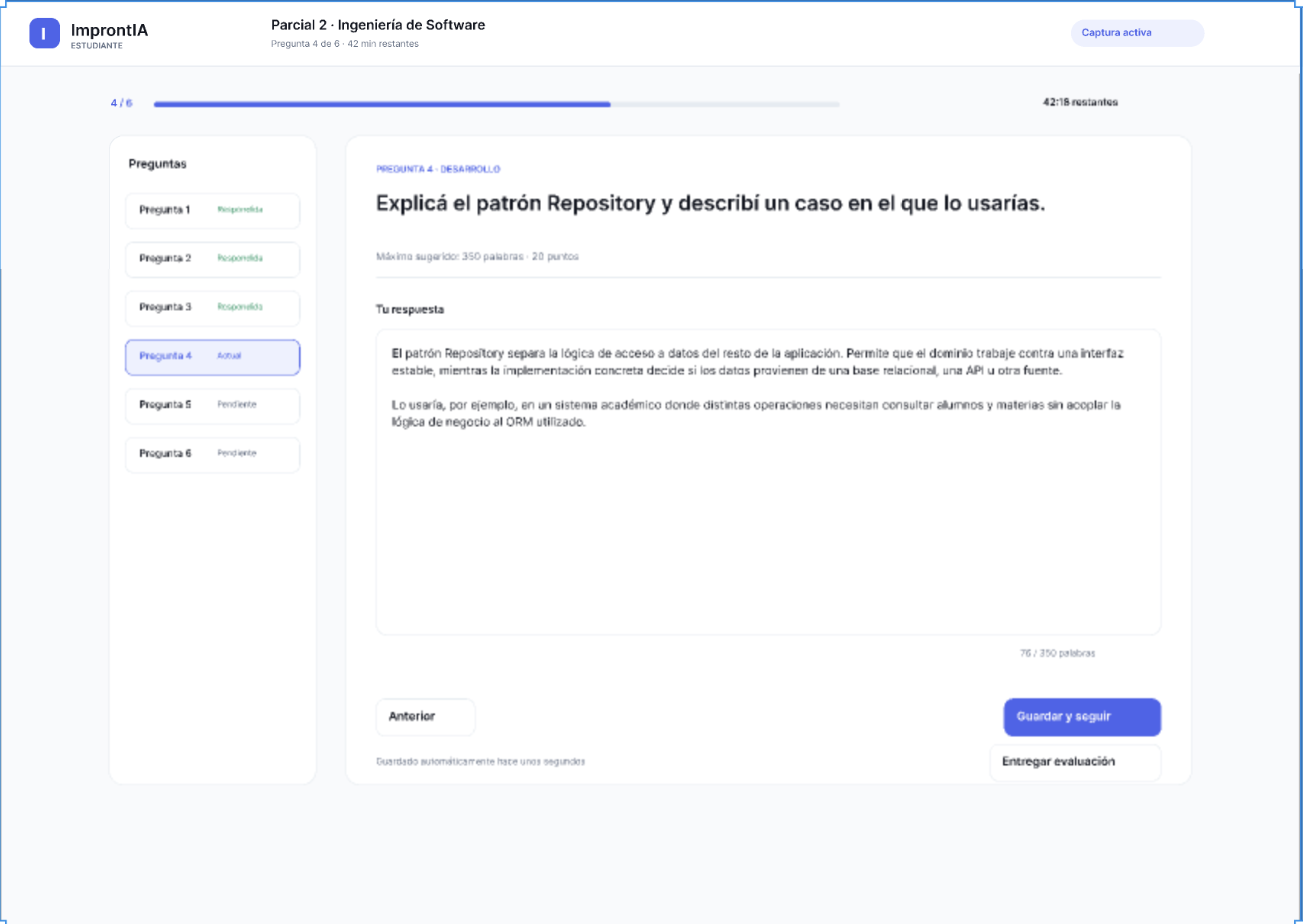
\includegraphics[width=0.85\textwidth]{./figures/mockup_estudiante_examen.png}
    \caption[Estudiante: evaluación en curso, con indicador de captura activa visible en todo momento]{Estudiante. Evaluación en curso, con indicador de captura activa visible en todo momento. Fuente: elaboración propia (prototipo diseñado en Figma).}
\end{figure}

El prototipo completo tiene siete pantallas; además de las cinco reproducidas, incluye \textit{Registrar revisión} y \textit{Fin de sesión / Confirmación}, que el MVP implementa y se muestran en las capturas del Capítulo~\ref{ch:implementacion}.

El diseño refleja los principios de revisión humana (RF10) y de transparencia desarrollados en este capítulo: las pantallas del docente presentan señales e indicadores como evidencia revisable y trazable hasta su origen (RF06--RF09).

